\chapter{Experimental Apparatus}
\label{CHAPTER:ExperimentalApparatus}

%%%%%%%%%%%%%%%%%%%%%%%%%%%%%%%%%%%%%%%%%%%%%%%%%%%%%%%%%%%%%%%%%%%%%%%%%%%%%%%%%%%%%%%
%%% SECTION
%%%%%%%%%%%%%%%%%%%%%%%%%%%%%%%%%%%%%%%%%%%%%%%%%%%%%%%%%%%%%%%%%%%%%%%%%%%%%%%%%%%%%%%
\section{The Large Hadron Collider}
\label{SECTION:ExperimentalApparatus_LHC}

% Status: Writing
%
% TODO:
% * DONE: LHC location, size, particles used, energy usage.
% * Basics of machine and operation
% * How instantaneous luminosity is calculated include Instantaneous luminosity equation
% * Delivered instantaneous luminosity Run I (proton-Proton)

% \colorbox{red}{
% \begin{minipage}{0.95\linewidth}
%  
% \begin{itemize}\item\end{itemize}
% \end{minipage}
%}

The \gls{LHC}\cite{ARTICLE:LHC Machine} is currently the world's largest particle accelerator and is capable to produce the highest energy particle beam ever made by mankind. This gigantic machine with a total perimeter of 26.7 kilometer was built at \gls{CERN} in a circular tunnel at an average depth of 100 meters below ground under the Franco-Swiss border near Geneva, Switzerland. I Diagram of the LHC tunnel can be found in figure \ref{FIGURE:ExperimentalApparatus_LHCLayoutUnderground}.

\begin{figure}[!htb]
  \centering
  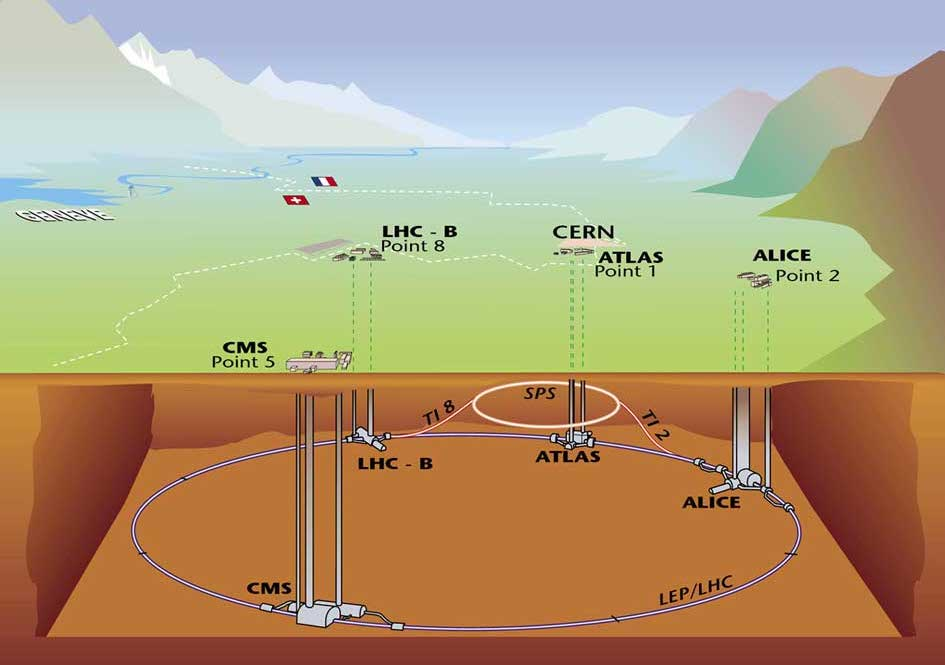
\includegraphics[width=0.50\textwidth]{Chapter02/LHC/Images/LHC_layout_underground.jpg}
  \caption{Underground diagram of the Geneva area showing the \gls{LHC} location.}
  \label{FIGURE:ExperimentalApparatus_LHCLayoutUnderground}
\end{figure}

The \gls{LHC} is a synchrotron machine with the capability to accelerate particles in two separated beam pipes with travel in opposite direction.  These beams only cross and are allowed to collide in four specific points of the accelerator where huge particle detectors are installed to detect the products of such collisions. This experiments are name ATLAS\cite{ARTICLE:TheATLASExperiment}, CMS\cite{ARTICLE:TheCMSExperiment}, LHCb\cite{ARTICLE:TheLHCbExperiment} and ALICE\cite{ARTICLE:TheALICEExperiment}.

The accelerator as its name indicates can collide hadrons, more specifically proton or heavy ions. Up to now 3 modes of operation have been tried according to the particles being collided: proton-proton, proton-lead and lead-lead. Depending on the which configuration is chosen we are basically changing the quantity of nucleons available to each colliding element. The maximum design energy per proton is 7 TeV and for each lead nucleon 2.76 TeV. The design luminosity for proton-proton is of $10^{34}$ $cm^{-2}s^{-1}$ and for lead-lead is of $10^{27}$ $cm^{-2}s^{-1}$.

The \gls{LHC} is only the last element of a complex accelerator chain which step by step increases the energy of the particles. Protons are initially obtained by stipping the electrons of hydrogen gas. The are then accelerated at the \gls{LINAC2} up to the energy of 50 MeV. After this initial step they are injected into the \gls{PSB} and the energy ramps ups to 1.4 GeV. After protons are passed to the \gls{PS} where energy futher increases to 25 GeV subsequently they are the injected into the \gls{SPS} where the particle energy level reached 450 GeV. Finally, protons pass to the \gls{LHC} where they can be accelerated to a maximum energy of 7 TeV. A simplified diagram of the \gls{CERN} accelerator chain can be found in figure \ref{FIGURE:ExperimentalApparatus_LHCAccelaratorChain}.

\begin{figure}[!htb]
  \centering
  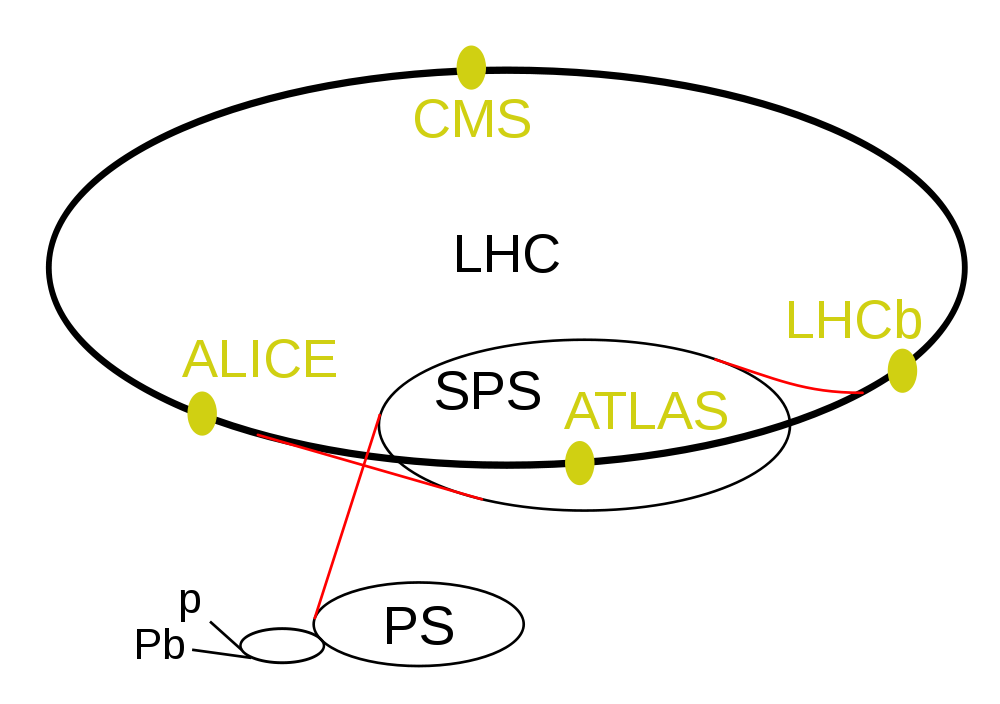
\includegraphics[width=0.50\textwidth]{Chapter02/LHC/Images/LHCAccelaratorChain.png}
  \caption{CERN Large Hadron Collider Experiment accelerator diagram.}
  \label{FIGURE:ExperimentalApparatus_LHCAccelaratorChain}
\end{figure}

Normal operation of the \gls{LHC} therefore depends on the the upstream accelerators availability. The typically turn around time, the time necessary to stop the accelerator from running and restart collisions is around 2 hours. When stable beams are achieved, a single proton fill can be used to collide protons up to 24 hours, but it is common to restart more frequently to take profit of the higher collision rates possible right at the beginning of a new fill.

Some of the key parameters of the LHC proton-proton and lead-lead operation can be found in table \ref{TABLE:ExperimentalApparatus_LHCMachineParameters}.

\begin{table}[!htb]
  \centering
  \begin{threeparttable}
    \begin{tabular}{|lcccc|}
    \hline 
                                  &              &           \textit{pp} &         \textbf{HI} &  \\
    \hline\hline
    Energy per nucleon            & E            &                     7 &                2.76 &                 $\TeV$ \\
    Dipole field at 7 TeV         & \textit{B}   &                  8.33 &                8.33 &               $\tesla$ \\
    Design Luminosity\tnote{*}    & $\mathcal{L}$ &            $10^{34}$ &           $10^{27}$ & $\cm^{-2}\second^{-1}$ \\
    Bunch separation              &              &                    25 &                 100 &                  $\ns$ \\
    No. of bunches                & $k_B$        &                  2808 &                 592 &                        \\
    No. particles per bunch       & $N_p$        & $1.15 \times 10^{11}$ & $7.0 \times 10^{7}$ &                        \\
    \hline
    \hline
    \textbf{Collisions}           &              &  &  &  \\
    \hline
    $\beta$-value at IP           & $\beta^{*}$  &                  0.55 &                 0.5 &        $\meter$ \\
    RMS beam radius at IP         & $\sigma^{*}$ &                  16.7 &                15.9 &  $\micro\meter$ \\
    Luminosity lifetime           & $\tau_L$     &                    15 &                   6 &         $\hour$ \\
    Number of collisions/crossing & $n_c$        &          $\approx 20$ &                   - &                 \\
    \hline
    \end{tabular}
    \begin{tablenotes}
      \item[*] For heavy-ion (HI) operation the design luminosity for Pb-Pb collisions is given.
    \end{tablenotes}
  \end{threeparttable}
  \caption[LHC parameters relevant for detectors]{The machine parameters relevant for the 
                                                  LHC detectors.\cite{CMSTDR:CMSPhysicsVol1}}
  \label{TABLE:ExperimentalApparatus_LHCMachineParameters}
\end{table}


\begin{figure}[!htb]
  \centering
  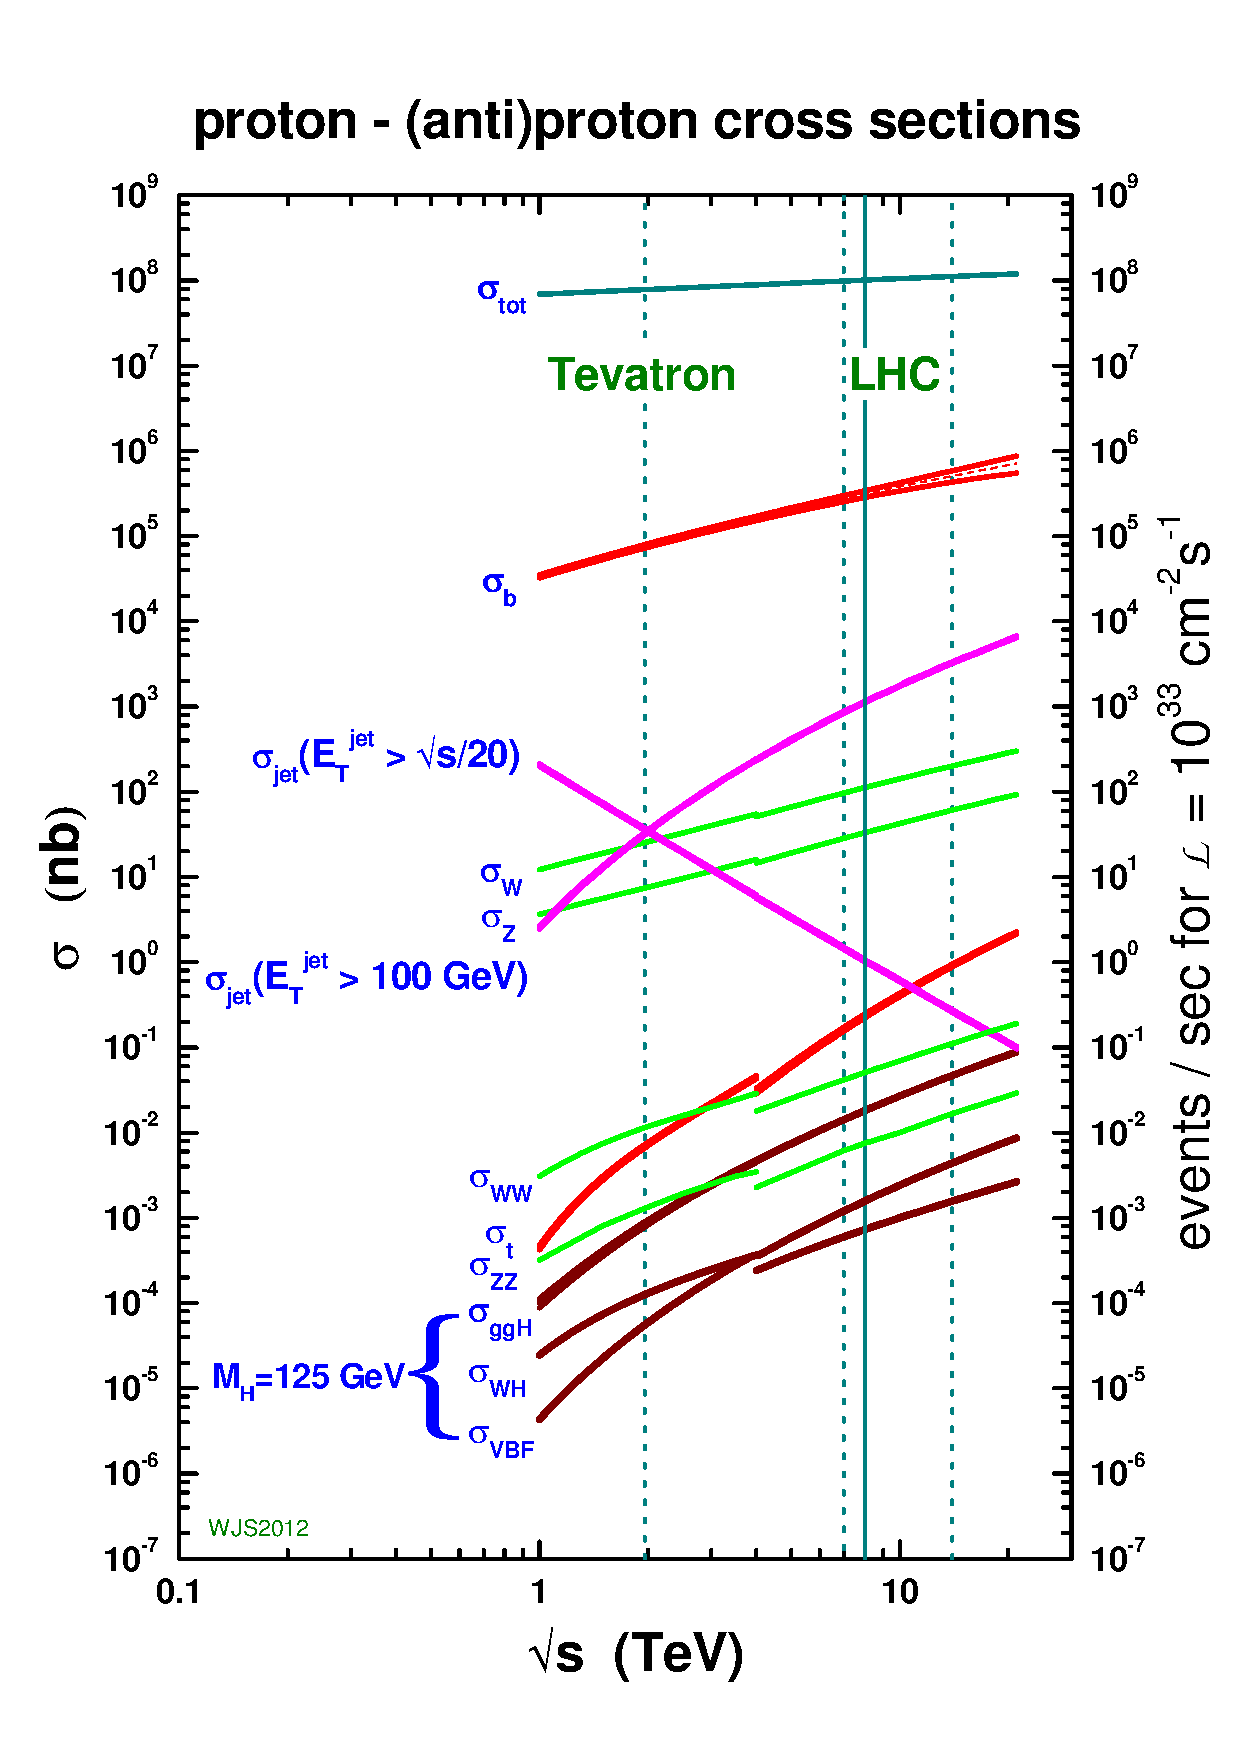
\includegraphics[width=0.50\textwidth]{Chapter02/LHC/Images/crosssections2012_v5}
  \caption{Cross sections for several processes for collisions of antiproton-proton and proton-proton as a function of the center of mass energy\cite{ARTICLE:TheCMSExperiment}.}
  \label{FIGURE:ExperimentalApparatus_LHCCrossSections}
\end{figure}

At the \gls{LHC} we are looking for extremely rare processes as is can be seen in figure \ref{FIGURE:ExperimentalApparatus_LHCCrossSections} the production cross section of a \gls{SM} Higgs boson is more than 9 orders of magnitude smaller than the total proton-proton cross section. 

To be able to record and study such rare processes we need to produce a significant amount of collisions. For this purpose the LHC was designed to operate at high instantaneous luminosity, L. This quantity is defined as,

\begin{equation}
L=\frac{N_{b}^{2}n_{b}f_{\text{rev}}\gamma}{4\pi\epsilon_{n}\beta^{*}}F,
\end{equation}

where $N_{b}$ is the number of protons per bunch, $n_{b}$ is the number of bunches, $f_{\text{rev}}$ is the frequency of revolution, $\gamma$ is the Lorentz factor, $\epsilon_{n}$ is the normalized emittance, $f_{\text{rev}}$ is the beta function at the collision point and $F$ is the reduction factor due to the crossing angle.

%%%%%%%%%%%%%%%%%%%%%%%%%%%%%%%%%%%%%%%%%%%%%%%%%%%%%%%%%%%%%%%%%%%%%%%%%%%%%%%%%%%%%%%
%%% SUBSECTION
%%%%%%%%%%%%%%%%%%%%%%%%%%%%%%%%%%%%%%%%%%%%%%%%%%%%%%%%%%%%%%%%%%%%%%%%%%%%%%%%%%%%%%%
\subsection{Delivered Luminosity}

\begin{figure}[!htb]
  \centering
  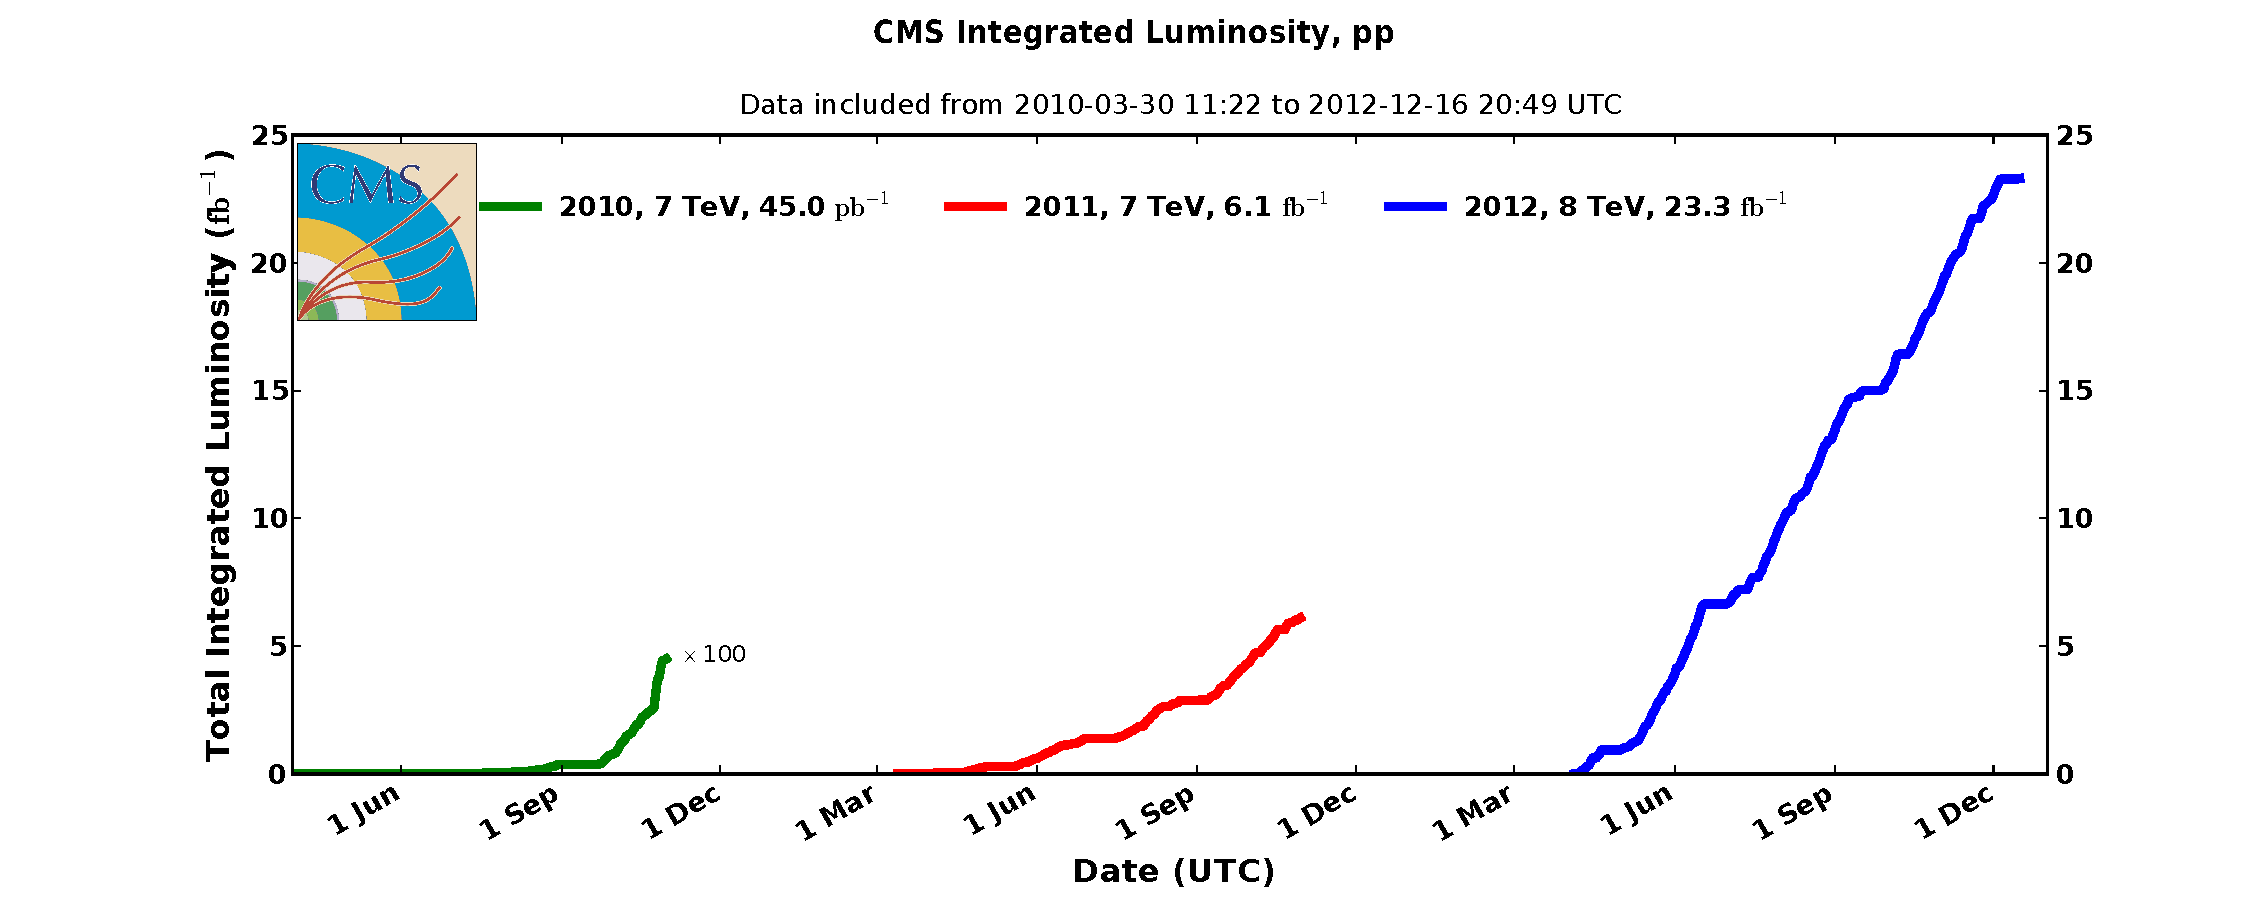
\includegraphics[width=1.00\textwidth]{Chapter02/CMS/Images/CMS_IntegratedLumi_pp_2010-2012}
  \caption{Cumulative luminosity versus day delivered to CMS during stable beams and for p-p collisions. This is shown for 2010 (green), 2011 (red) and 2012 (blue) data-taking.}
  \label{FIGURE:ExperimentalApparatus_CMS_IntegratedLumi_pp_2010-2012}
\end{figure}

\begin{figure}[!htb]
  \centering
  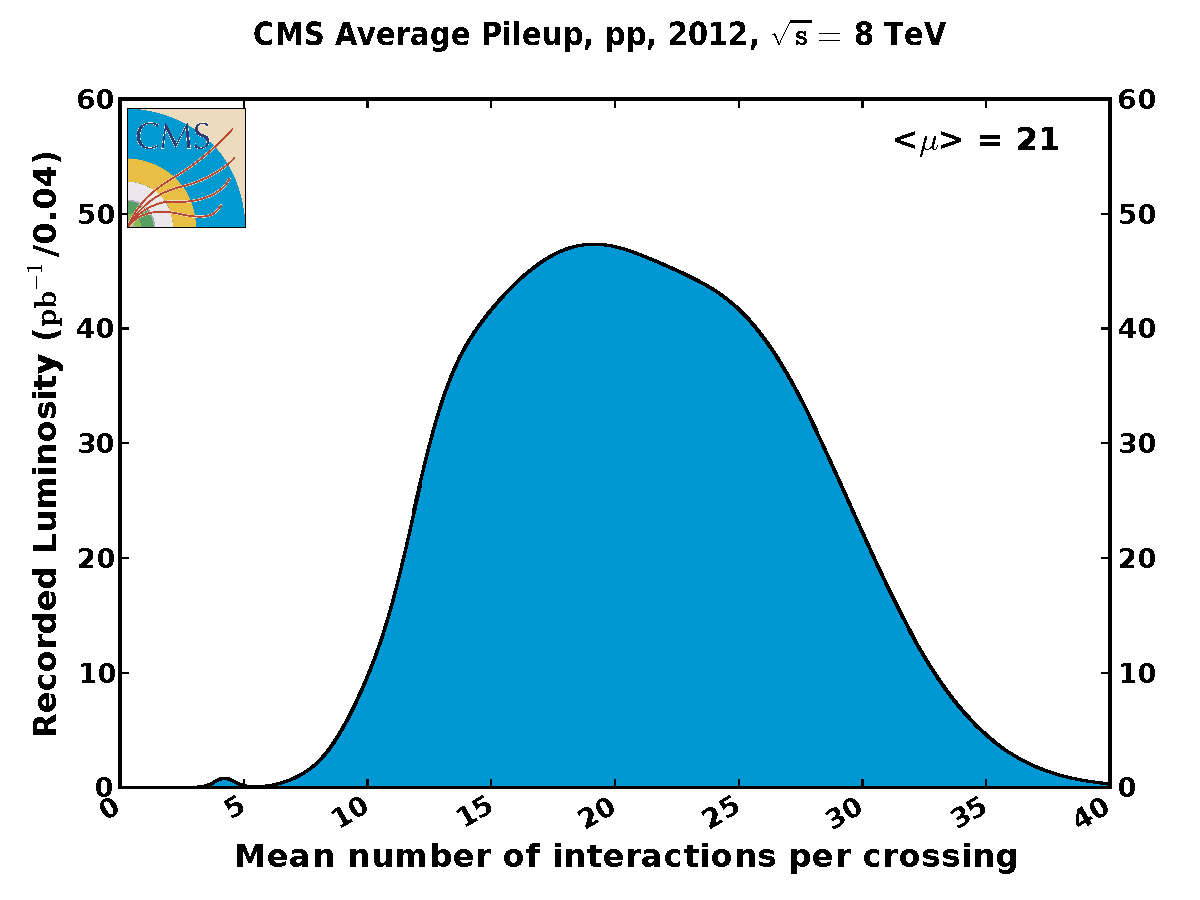
\includegraphics[width=0.50\textwidth]{Chapter02/CMS/Images/CMS_PileIp_pp_2012}
  \caption{Mean number of interactions per bunch crossing at the CMS experiment during 2012.}
  \label{FIGURE:ExperimentalApparatus_CMS_PileIp_pp_2012}
\end{figure}

\section{The Compact Muon Solenoid Experiment}
\label{SECTION:ExperimentalApparatus_CMS}

The \gls{CMS} experiment is a general purpose experiment located at point 5 of the \gls{LHC}. It was designed to study collisions at its centre and is composed os several sub-systems in an classic onion shaped structure.


%%%%%%%%%%%%%%%%%%%%%%%%%%%%%%%%%%%%%%%%%%%%%%%%%%%%%%%%%%%%%%%%%%%%%%%%%%%%%%%%%%%%%%%
%%% SUBSECTION
%%%%%%%%%%%%%%%%%%%%%%%%%%%%%%%%%%%%%%%%%%%%%%%%%%%%%%%%%%%%%%%%%%%%%%%%%%%%%%%%%%%%
\subsection{Geometry and conventions}


%%%%%%%%%%%%%%%%%%%%%%%%%%%%%%%%%%%%%%%%%%%%%%%%%%%%%%%%%%%%%%%%%%%%%%%%%%%%%%%%%%%%%%%
%%% SUBSECTION
%%%%%%%%%%%%%%%%%%%%%%%%%%%%%%%%%%%%%%%%%%%%%%%%%%%%%%%%%%%%%%%%%%%%%%%%%%%%%%%%%%%%
\subsection{Inner tracking system}
\label{SUBSECTION:ExperimentalApparatus_CMS_Tracker}

% STATUS: DONE (reviwed J.Pela x1)
%
% Writing points:
% * Closest detector to beam, measures trajectories of charged particles
% * With magnetic field measures momentum and charge of this particles
% * Allows vertexing (primary and secundary)
% * Different regions different occupancy
% * Final arranagement

The inner tracking system is the closest detector to the beam axis and the interaction region. Its function is to measure the trajectory of all charged particles, like electrons, charged hadrons and muons with momentum above 1 $GeV$ being produced at each \gls{LHC} collision. With the help of the strong magnetic field produced by the \gls{CMS} magnet particle trajectories are bent allowing for charge and momentum determination. With the resulting tracks is it then possible to determine the primary vertex as well as secondary vertexes like other lower energy proton-proton collision or displaced vertexes from the decay of long lived particles like B mesons.

Building a tracking system for an experiment at the \gls{LHC} is very challenging. At design luminosity an average of 1000 particles will hit such system at a rate approaching 40 $MHz$, leading to high hit density at high rate. It is therefore desirable to have a fast, efficient and high granularity detector where at each layer the occupancy should be at or below $1\%$. On the other hand each layer should be as thin as possible in order to not change the incoming particles trajectory or make them lose too much energy. The detector should also be radiation hard and survive for a period of at least 10 years due to its importance and location. This design requirements have lead to a tracker design entirely based on silicon detector technology. 

The volume near the interaction point can be split according to the charged particle flux into three regions:

\begin{itemize}
  \item $r<10$ $cm$: highest particle flux, up to $\approx 10^8 $ $cm^{-2}s^{-1}$ at $r \approx 4$ $cm$, pixel detectors are used. The pixel size is $\approx 100 \times 150$ $\mu m^2$, which translates into an occupancy of $10^{-4}$ per \gls{LHC} bunch crossing.
  \item $20<r<55$ $cm$: particle flux decreases enough to use silicon micro-strips with a minimum cell size of 10 cm $\times$ 80 $\mu m$, leading to an occupancy of $\approx 2-3\%$ per \gls{LHC} bunch crossing.
  \item $50<r<110$ $cm$: most outer region of the tracker, particle flux is low enough to use larger pitch silicon micro-strips. The maximum cell size is of 25 $cm$ $\times$ 180 $\mu m$, and occupancy is of the order of $\approx 1\%$.
\end{itemize}

The \gls{CMS} tracker final configuration is composed of a pixel detector with three barrel layers at radii between 4.4 $cm$ and 10.2 $cm$ and 2 disks on each side of the barrel. And a silicon strip tracker with 10 barrel detection layers extending up to 1.1 $m$ with 3 plus 9 disks on each side of the barrel. A schematic of the detector module distribution can be found at figure \ref{FIGURE:ExperimentalApparatus_CMS_Tracker_Layout}. This detector has an acceptance covering up to pseudorapidity of $|\eta|<2.5$ and has a total active area of about 200 $m^2$ making the largest silicon tracker ever built. 

\begin{figure}[!htb]
  \centering
  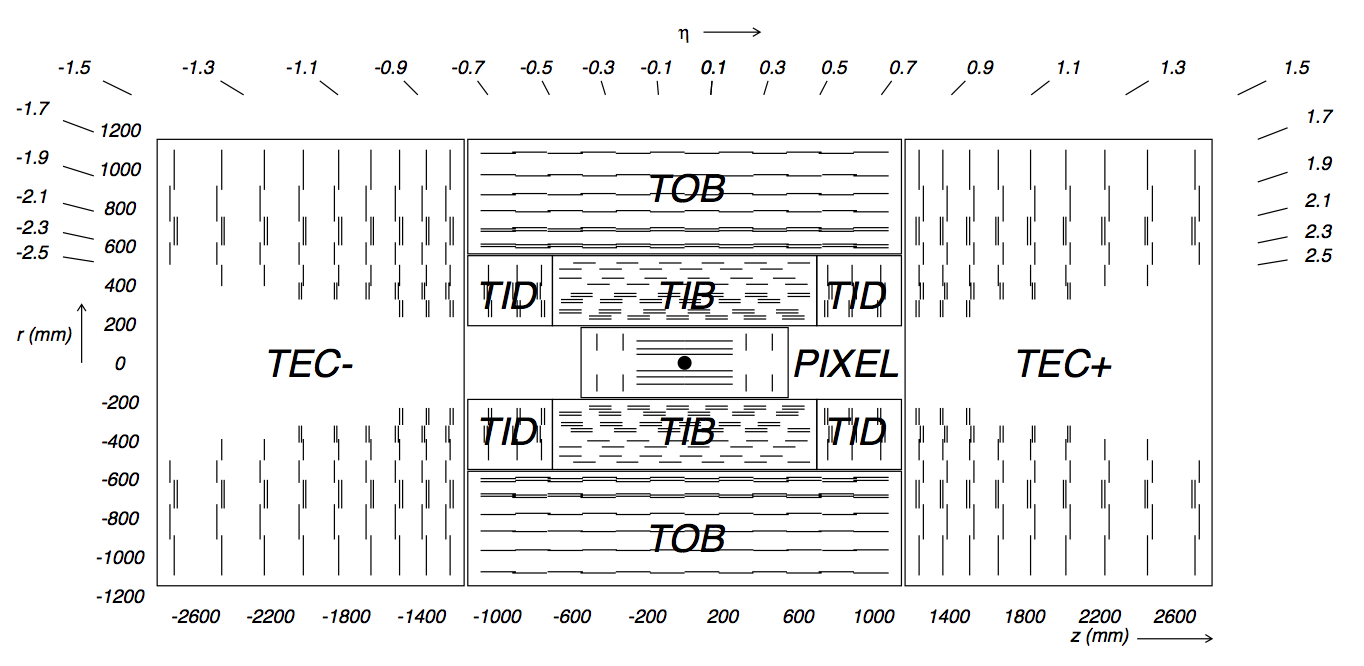
\includegraphics[width=1.0\textwidth]{Chapter02/CMS/Images/CMS_Tracker_Layout.png}
  \caption{Schematic cross section of the CMS tracker. Each line represent a detector module. Double lines represent dual surface back-to-back detector modules.}
  \label{FIGURE:ExperimentalApparatus_CMS_Tracker_Layout}
\end{figure}

%%%%%%%%%%%%%%%%%%%%%%%%%%%%%%%%%%%%%%%%%%%%%%%%%%%%%%%%%%%%%%%%%%%%%%%%%%%%%%%%%%%%%%%
%%% SUBSECTION
%%%%%%%%%%%%%%%%%%%%%%%%%%%%%%%%%%%%%%%%%%%%%%%%%%%%%%%%%%%%%%%%%%%%%%%%%%%%%%%%%%%%
\subsection{Electromagnetic Calorimeter}
\label{SUBSECTION:ExperimentalApparatus_CMS_ECAL}

% Status: DONE (just with MSc input, and needs review)

The \gls{ECAL} is an hermetic energy measurement system comprised of 61200 lead tungstate ($PbWO_4$) crystals mounted in the barrel and 7324 crystals in each of the 2 endcaps.

Lead tungstate has a fairly high density (8.28 $g/cm^3$), has a short radiation length (0.89 $cm$) and a small Moliere redius (2.2 $cm$). The crystals also have a fast scintillation decay time emitting 80\% of the light yield in 25 $ns$ (the minimal bunch crossing time at the LHC). This characteristics make it a good choice for an electromagnetic calorimeter allowing a compact design with fine granularity. However, this crystals emit a fairly low light yield (30 $\gamma/MeV$) which requires the use of photo-detectors with intrinsic gain which will preform well inside a magnitic field. In the barrel region silicon \gls{APD} are used and \gls{VPT} are used in the endcaps. To guarantee good response from both crystals and \gls{APD} it is necessary to have system thermal stability, with the goal being temperature variation of less than 0.1º C.

The barrel section, the \gls{EB}, has an inner radius of 129 $cm$ and is composed of 36 identical ``supermodules``, each covers the barrel length and corresponding to a pseudo-rapidity interval of $0<|\eta|<1.479$. The crystals are quasi-projective (the axes are tilted at 3º with respect to the line from the nominal vertex position) and cover 0.0174 (i.e. 1º ) in $\Delta\phi$ and $\Delta\eta$. The crystals have a front face cross-section of $\approx 22\times22$ $mm^2$ and a length of 230 $mm$, corresponding to 25.8 $X_0$.

The endcap section, the \gls{EE}, is at a distance of 314 cm from the vertex and covering a pseudorapidity range of $1.479<|\eta|<3.0$, are each structured as 2 “Dees”, consisting of semi-circular aluminium plates from which are cantilevered structural units of $5\times5$ crystals, known as “supercrystals”.

figure \ref{FIGURE:ExperimentalApparatus_CMS_ECAL_Layout}

\begin{figure}[!htb]
  \centering
  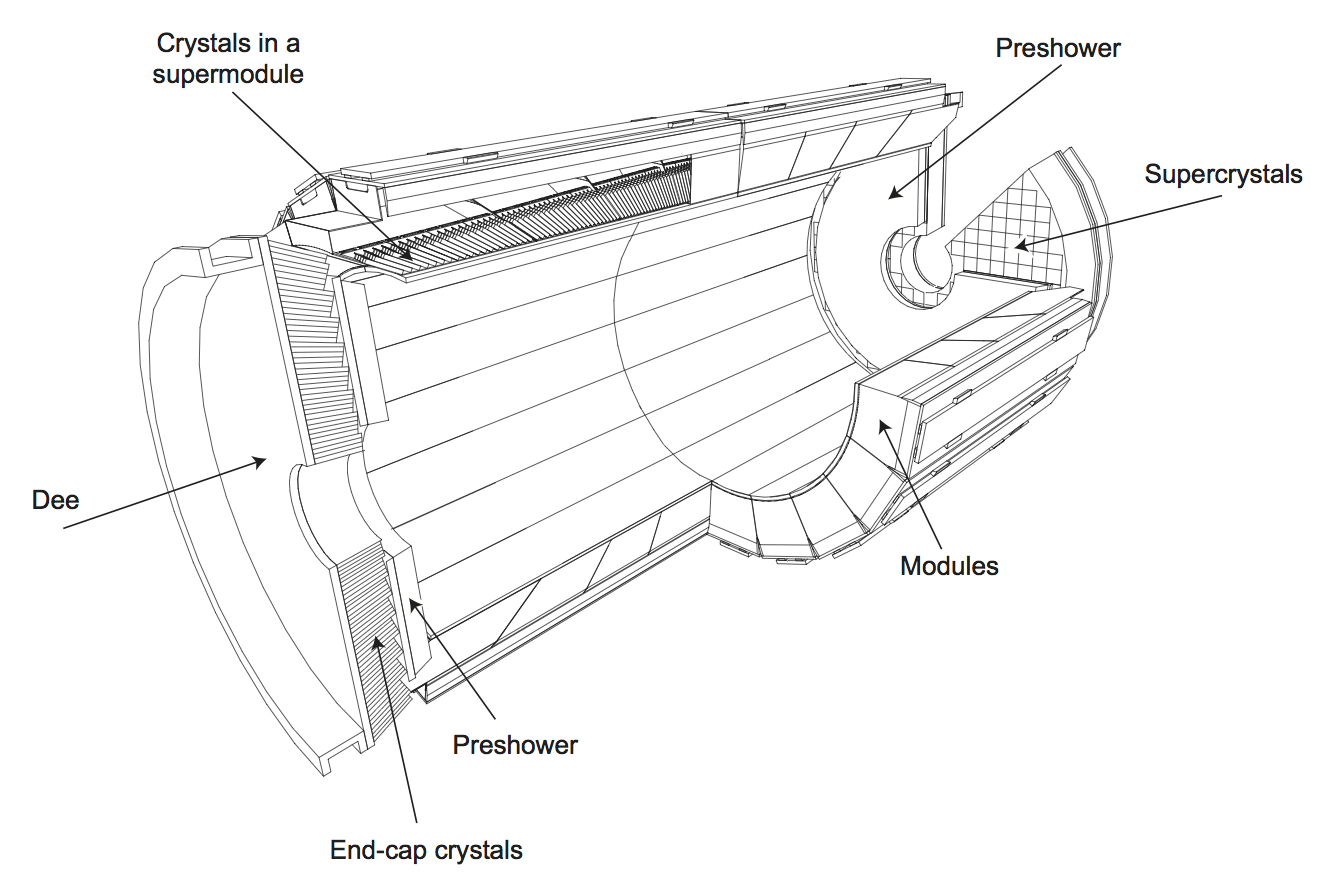
\includegraphics[width=1.0\textwidth]{Chapter02/CMS/Images/CMS_ECAL_Layout.png}
  \caption{}
  \label{FIGURE:ExperimentalApparatus_CMS_ECAL_Layout}
\end{figure}


%%%%%%%%%%%%%%%%%%%%%%%%%%%%%%%%%%%%%%%%%%%%%%%%%%%%%%%%%%%%%%%%%%%%%%%%%%%%%%%%%%%%%%%
%%% SUBSECTION
%%%%%%%%%%%%%%%%%%%%%%%%%%%%%%%%%%%%%%%%%%%%%%%%%%%%%%%%%%%%%%%%%%%%%%%%%%%%%%%%%%%%
\subsection{Hadronic Calorimeter}
\label{SUBSECTION:ExperimentalApparatus_CMS_HCAL}

% STATUS: Writing

The \gls{HCAL} is a sampling calorimeter which is designed to measure the properties of hadron jets and indirectly neutrinos or other undiscovered particles that would result in apparent missing energy\cite{ARTICLE:CMSTechnicalProposal}. 

The design of the \gls{HCAL} was strongly influenced by the choice of the magnet parameters since most of the calorimetry is inside of the magnet. The \gls{HB} is limited from the beam side by the \gls{ECAL} at radius $r=1.77$ $m$ and outwards by the magnet at radius $r=2.95$ $m$. This is a strict limitation on the amount of absorber material to be used. To improve the measurement capability, an outer calorimeter, the \gls{HO}, is placed outside of the magnet as a \textit{tail catcher} outside of the solenoid magnet. Closing the barrel in each side the \gls{HE} are present with acceptance up to pseudorapidity $|\eta|<3$.  
Additionally, to extend acceptance to $|\eta|<5.2$ the \gls{HF} is installed at 11.2 $m$ from the interaction point providing excellent hermeticity for $E_{\perp}^{miss}$ measurement. A diagram of the \gls{HCAL} subsystems and their location inside \gls{CMS} can be found in figure \ref{FIGURE:ExperimentalApparatus_CMS_HCAL_Layout}.

\begin{figure}[!htb]
  \centering
  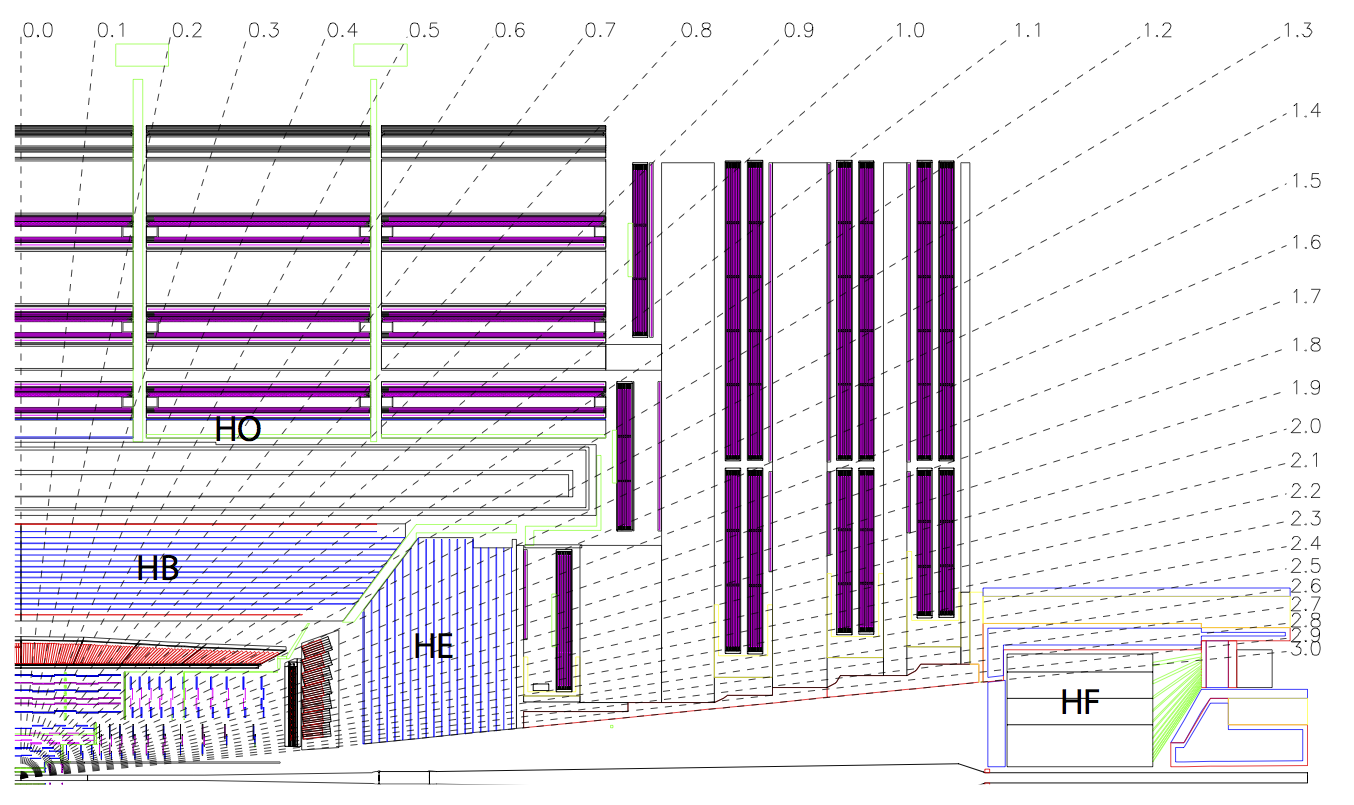
\includegraphics[width=1.0\textwidth]{Chapter02/CMS/Images/CMS_HCAL_Layout.png}
  \caption{Longitudinal view of the CMS detector highlighting the location of the \gls{HCAL} components: \gls{HB}, \gls{HE} \gls{HO} and \gls{HF}.}
  \label{FIGURE:ExperimentalApparatus_CMS_HCAL_Layout}
\end{figure}

The \gls{HB} covers the region up to $|\eta|<1.3$ and divided into towers with segmentation of $\Delta\eta \times \Delta\phi = 0.087 \times 0.087$ which corresponds to the same area of a $5 \times 5$ arrays of \gls{ECAL} crystals. 
% Alternated layers of scintillators and absorver
% Brass absorver (shoter interaction lenght (16.42 cm ref?) and is non magnetic.
% Hadrons cause light pulses in the plastic fibers which go to hybrid photo diodes via wavelenght-shifting fibers.


The \gls{HO}


The \gls{HB} covers the range of $1.3<|\eta|<3.0$...


The \gls{HF} covers the range of $3.0<|\eta|<5.2$...
% higest flux
% made of radiation hard quartz fibers (active medium), steel absorver
% Cherenkov radiation from particles in fibers gives signal


% Brass has been chosen as absorber material as it has a reasonably short interaction length, is easy to machine and is non-magnetic. The overall assembly enables the HCAL to be built with essentially no uninstrumented cracks or dead
% areas in φ. The gap between the barrel and the endcap HCAL, through which the services of the ECAL and the inner tracker pass, is inclined at 53o and points away from the center of the detector. The hadron barrel (HB) part of HCAL consists of 32 towers covering the pseudorapidity region −1.4 <
% η < 1.4, resulting in 2304 towers with a segmentation ∆η×∆φ = 0.087×0.087. The HB is constructed in 2 half barrels.
% 10
% The hadron outer (HO) detector contains scintillators with a thickness of 10 mm, which line the outside
% of the outer vacuum tank of the coil and cover the region −1.26 < η < 1.26. The tiles are grouped in 30o-sectors, matching the φ segmentation of the DT chambers. They sample the energy from penetrating
% hadron showers leaking through the rear of the calorimeters and so serve as a “tail-catcher” after the magnet coil.
% Each hadron endcap (HE) of HCAL consists of 14 η towers with 5o φ segmentation, covering the pseudo-
% rapidity region 1.3 < |η| < 3.0. For the 5 outermost towers (at smaller η) the φ segmentation is 5o and the η segmentation is 0.087. For the 8 innermost towers the φ segmentation is 10o , whilst the η segmentation
% varies from 0.09 to 0.35 at the highest η. The total number of HE towers is 2304. Coverage between pseudorapidities of 3.0 and 5.0 is provided by the steel/quartz fibre Hadron Forward
% (HF) calorimeter. Because the neutral component of the hadron shower is preferentially sampled in the HF technology, this design leads to narrower and shorter hadronic showers and hence is ideally suited for the congested environment in the forward region. The front face is located at 11.2 m from the interaction point. The depth of the absorber is 1.65 m.

%%%%%%%%%%%%%%%%%%%%%%%%%%%%%%%%%%%%%%%%%%%%%%%%%%%%%%%%%%%%%%%%%%%%%%%%%%%%%%%%%%%%%%%
%%% SUBSECTION
%%%%%%%%%%%%%%%%%%%%%%%%%%%%%%%%%%%%%%%%%%%%%%%%%%%%%%%%%%%%%%%%%%%%%%%%%%%%%%%%%%%%
\subsection{Solenoid Magnet}
\label{SUBSECTION:ExperimentalApparatus_CMS_Magnet}

\begin{table}[!htb]
  \centering
  \begin{tabular}{|l|c|}
  \hline
  Parameter & Value \\
  \hline\hline
  Field           & 4 T \\
  Inner Bore      & 5.9 m \\
  Length          & 12.9 m \\
  Number of turns & 2168 \\
  Current         & 19.5 kA \\
  Stored Energy   & 2.7 GJ \\
  Hoop Stress     & 64 atm \\
  \hline
  \end{tabular}
  \caption[Parameters of the CMS superconducting solenoid]{Parameters of the CMS superconducting solenoid}
  \label{TABLE:ExperimentalApparatus_CMSMagnetParameters}
\end{table}


%%%%%%%%%%%%%%%%%%%%%%%%%%%%%%%%%%%%%%%%%%%%%%%%%%%%%%%%%%%%%%%%%%%%%%%%%%%%%%%%%%%%%%%
%%% SUBSECTION
%%%%%%%%%%%%%%%%%%%%%%%%%%%%%%%%%%%%%%%%%%%%%%%%%%%%%%%%%%%%%%%%%%%%%%%%%%%%%%%%%%%%
\subsection{Muon System}
\label{SUBSECTION:ExperimentalApparatus_CMS_Moun}

figure \ref{FIGURE:ExperimentalApparatus_CMS_Muon_Layout}

\begin{figure}[!htb]
  \centering
  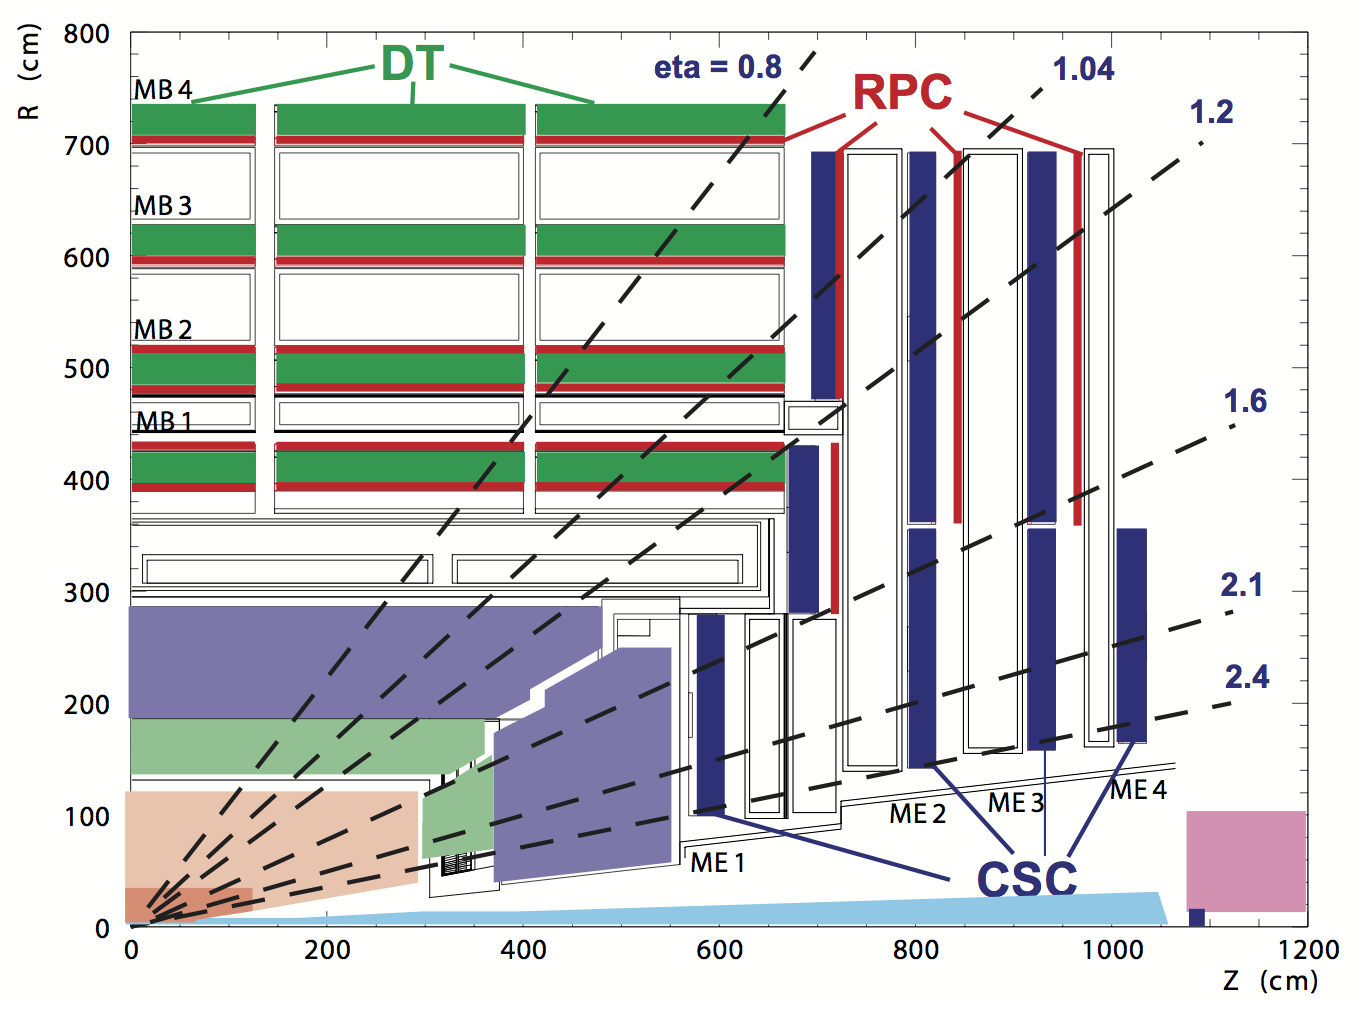
\includegraphics{Chapter02/CMS/Images/CMS_Muon_Layout.png}
  \caption{TODO}
  \label{FIGURE:ExperimentalApparatus_CMS_Muon_Layout}
\end{figure}

%%%%%%%%%%%%%%%%%%%%%%%%%%%%%%%%%%%%%%%%%%%%%%%%%%%%%%%%%%%%%%%%%%%%%%%%%%%%%%%%%%%%%%%
%%% SUBSECTION
%%%%%%%%%%%%%%%%%%%%%%%%%%%%%%%%%%%%%%%%%%%%%%%%%%%%%%%%%%%%%%%%%%%%%%%%%%%%%%%%%%%%
\subsection{Data Acquisition System}
\label{SUBSECTION:ExperimentalApparatus_CMS_DAQ}

The \gls{DAQ}

%%%%%%%%%%%%%%%%%%%%%%%%%%%%%%%%%%%%%%%%%%%%%%%%%%%%%%%%%%%%%%%%%%%%%%%%%%%%%%%%%%%%%%%
%%% SUBSECTION
%%%%%%%%%%%%%%%%%%%%%%%%%%%%%%%%%%%%%%%%%%%%%%%%%%%%%%%%%%%%%%%%%%%%%%%%%%%%%%%%%%%%
\subsection{Trigger System}
\label{SUBSECTION:ExperimentalApparatus_CMS_Trigger}

The \gls{L1T} and \gls{HLT}

CMS Tridas TDR\cite{CMSTDR:CMSTridasTDR} 

\begin{figure}[!htb]
  \centering
  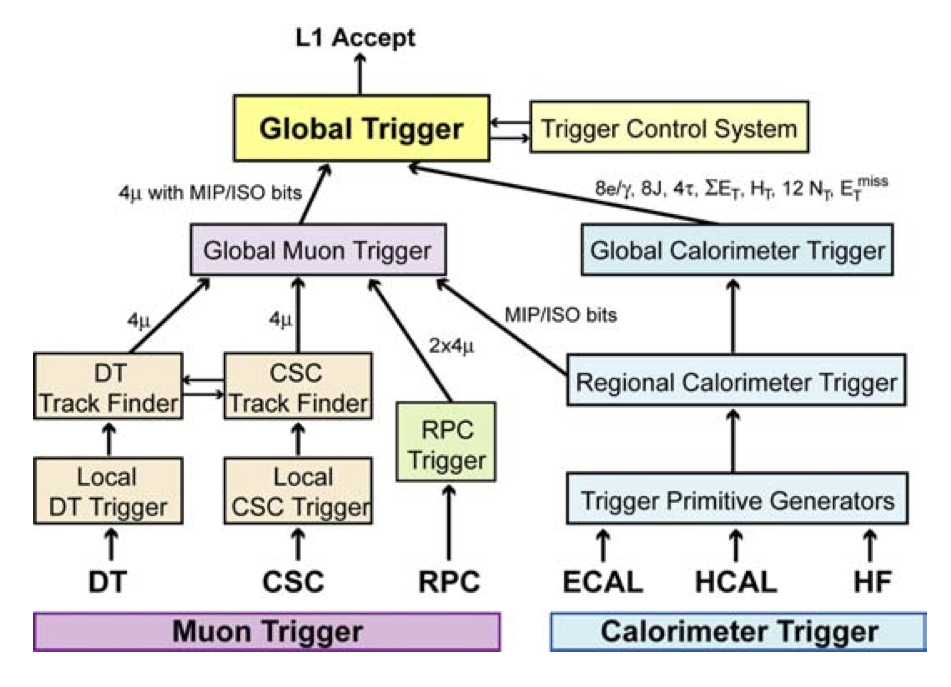
\includegraphics{Chapter02/CMS/Images/CMS_L1T_Layout.png}
  \caption{TODO}
  \label{FIGURE:ExperimentalApparatus_CMS_L1T_Layout}
\end{figure}

%%%%%%%%%%%%%%%%%%%%%%%%%%%%%%%%%%%%%%%%%%%%%%%%%%%%%%%%%%%%%%%%%%%%%%%%%%%%%%%%%%%%%%%
%%% SUBSECTION
%%%%%%%%%%%%%%%%%%%%%%%%%%%%%%%%%%%%%%%%%%%%%%%%%%%%%%%%%%%%%%%%%%%%%%%%%%%%%%%%%%%%
\subsection{Computing}
\label{SUBSECTION:ExperimentalApparatus_CMS_Computing}

The \gls{DQM} 

%%%%%%%%%%%%%%%%%%%%%%%%%%%%%%%%%%%%%%%%%%%%%%%%%%%%%%%%%%%%%%%%%%%%%%%%%%%%%%%%%%%%%%%
%%% SUBSECTION
%%%%%%%%%%%%%%%%%%%%%%%%%%%%%%%%%%%%%%%%%%%%%%%%%%%%%%%%%%%%%%%%%%%%%%%%%%%%%%%%%%%%
\subsection{Run II Upgrades}
\label{SUBSECTION:ExperimentalApparatus_CMS_RUNII}

CMS L1 Trigger Upgrade TDR\cite{CMSTDR:CMSL1Upgrade}
